\documentclass[ngerman,compress]{beamer}

\mode<presentation>
{
  \useoutertheme[footline=titleinstituteauthor]{c4}
  \useinnertheme{circles}
  \usecolortheme{c4}
  %\setbeamercovered{transparent}
  \setbeamercovered{highly dynamic}
}

\usepackage{babel}
\usepackage[utf8]{luainputenc}
\usepackage{fontspec}
\usepackage{listings}
\usepackage{color}


\title{U23 2013}

\author[andy <andy@koeln.ccc.de>, Florob <florob@babelmonkeys.de>] {andy, Florob}

\institute[Chaos Computer Club Cologne]
{
Chaos Computer Club Cologne e.V.\\
http://koeln.ccc.de \\
}

\date{2013-11-28}

\pgfdeclareimage[height=1cm]{barcode}{./c4-logo}
\logo{\pgfuseimage{barcode}}

\begin{document}

\begin{frame}
  \titlepage
\end{frame}

\AtBeginSubsection

%\begin{frame}
%  \tableofcontents
  % Die Option [pausesections] könnte nützlich sein.
%\end{frame}


\begin{frame}{U23 --- Was ist das?}
	\begin{itemize}
		\item Jugendprojekt des C4
		\item jährlich
		\item Teilnehmer bis 23 Jahre
		\item irgendwelche Soft-, oder Hardwareprojekte
	\end{itemize}
\end{frame}

\begin{frame}{Dieses Jahr}
	\begin{itemize}
		\item Mikrocontroller programmieren
		\item Über diverse Busse mit Peripherie reden
		\item Hardware: Grundplatine, diverse Sensoren (Distanz, Temperatur, Kompass, \ldots), diverse Ausgaben (LEDs, Displays, Servos, \ldots)
		\item Kleine Library, teils selbstgeschrieben, teils aus bestehenden zusammengeklaubt
	\end{itemize}
\end{frame}

\begin{frame}{Hardware: Grundplatine}
	\begin{columns}
		\column{0.5\textwidth}
			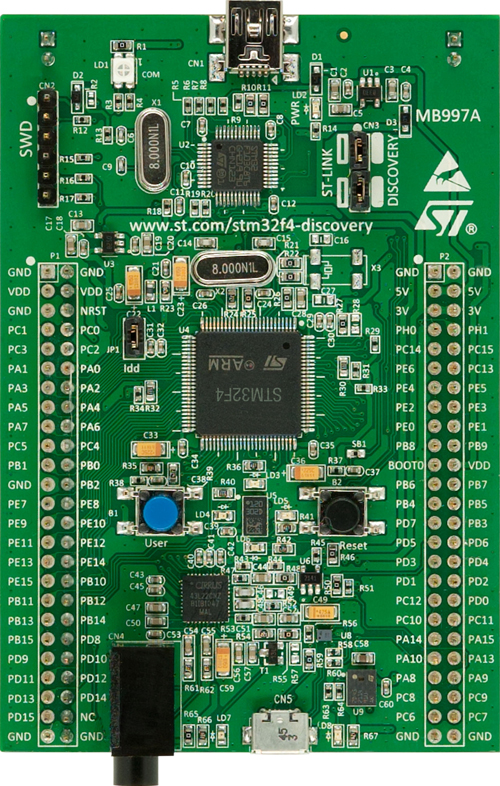
\includegraphics[width=0.4\textwidth]{stm32f4_discovery.jpg}
		\column{0.5\textwidth}
			\begin{itemize}
			\item STM32F407VGT6 32-bit ARM Cortex-M4F
			\item 1 MB Flash 
			\item 192 KB RAM
			\item JTAG via ST-Linkv2
			\item Audio Codec
			\item USB OTG
			\item 100pin LQFP
			\end{itemize}
	\end{columns}
\end{frame}

\begin{frame}{Bauteile}
	\begin{figure}[h]
		\centering
		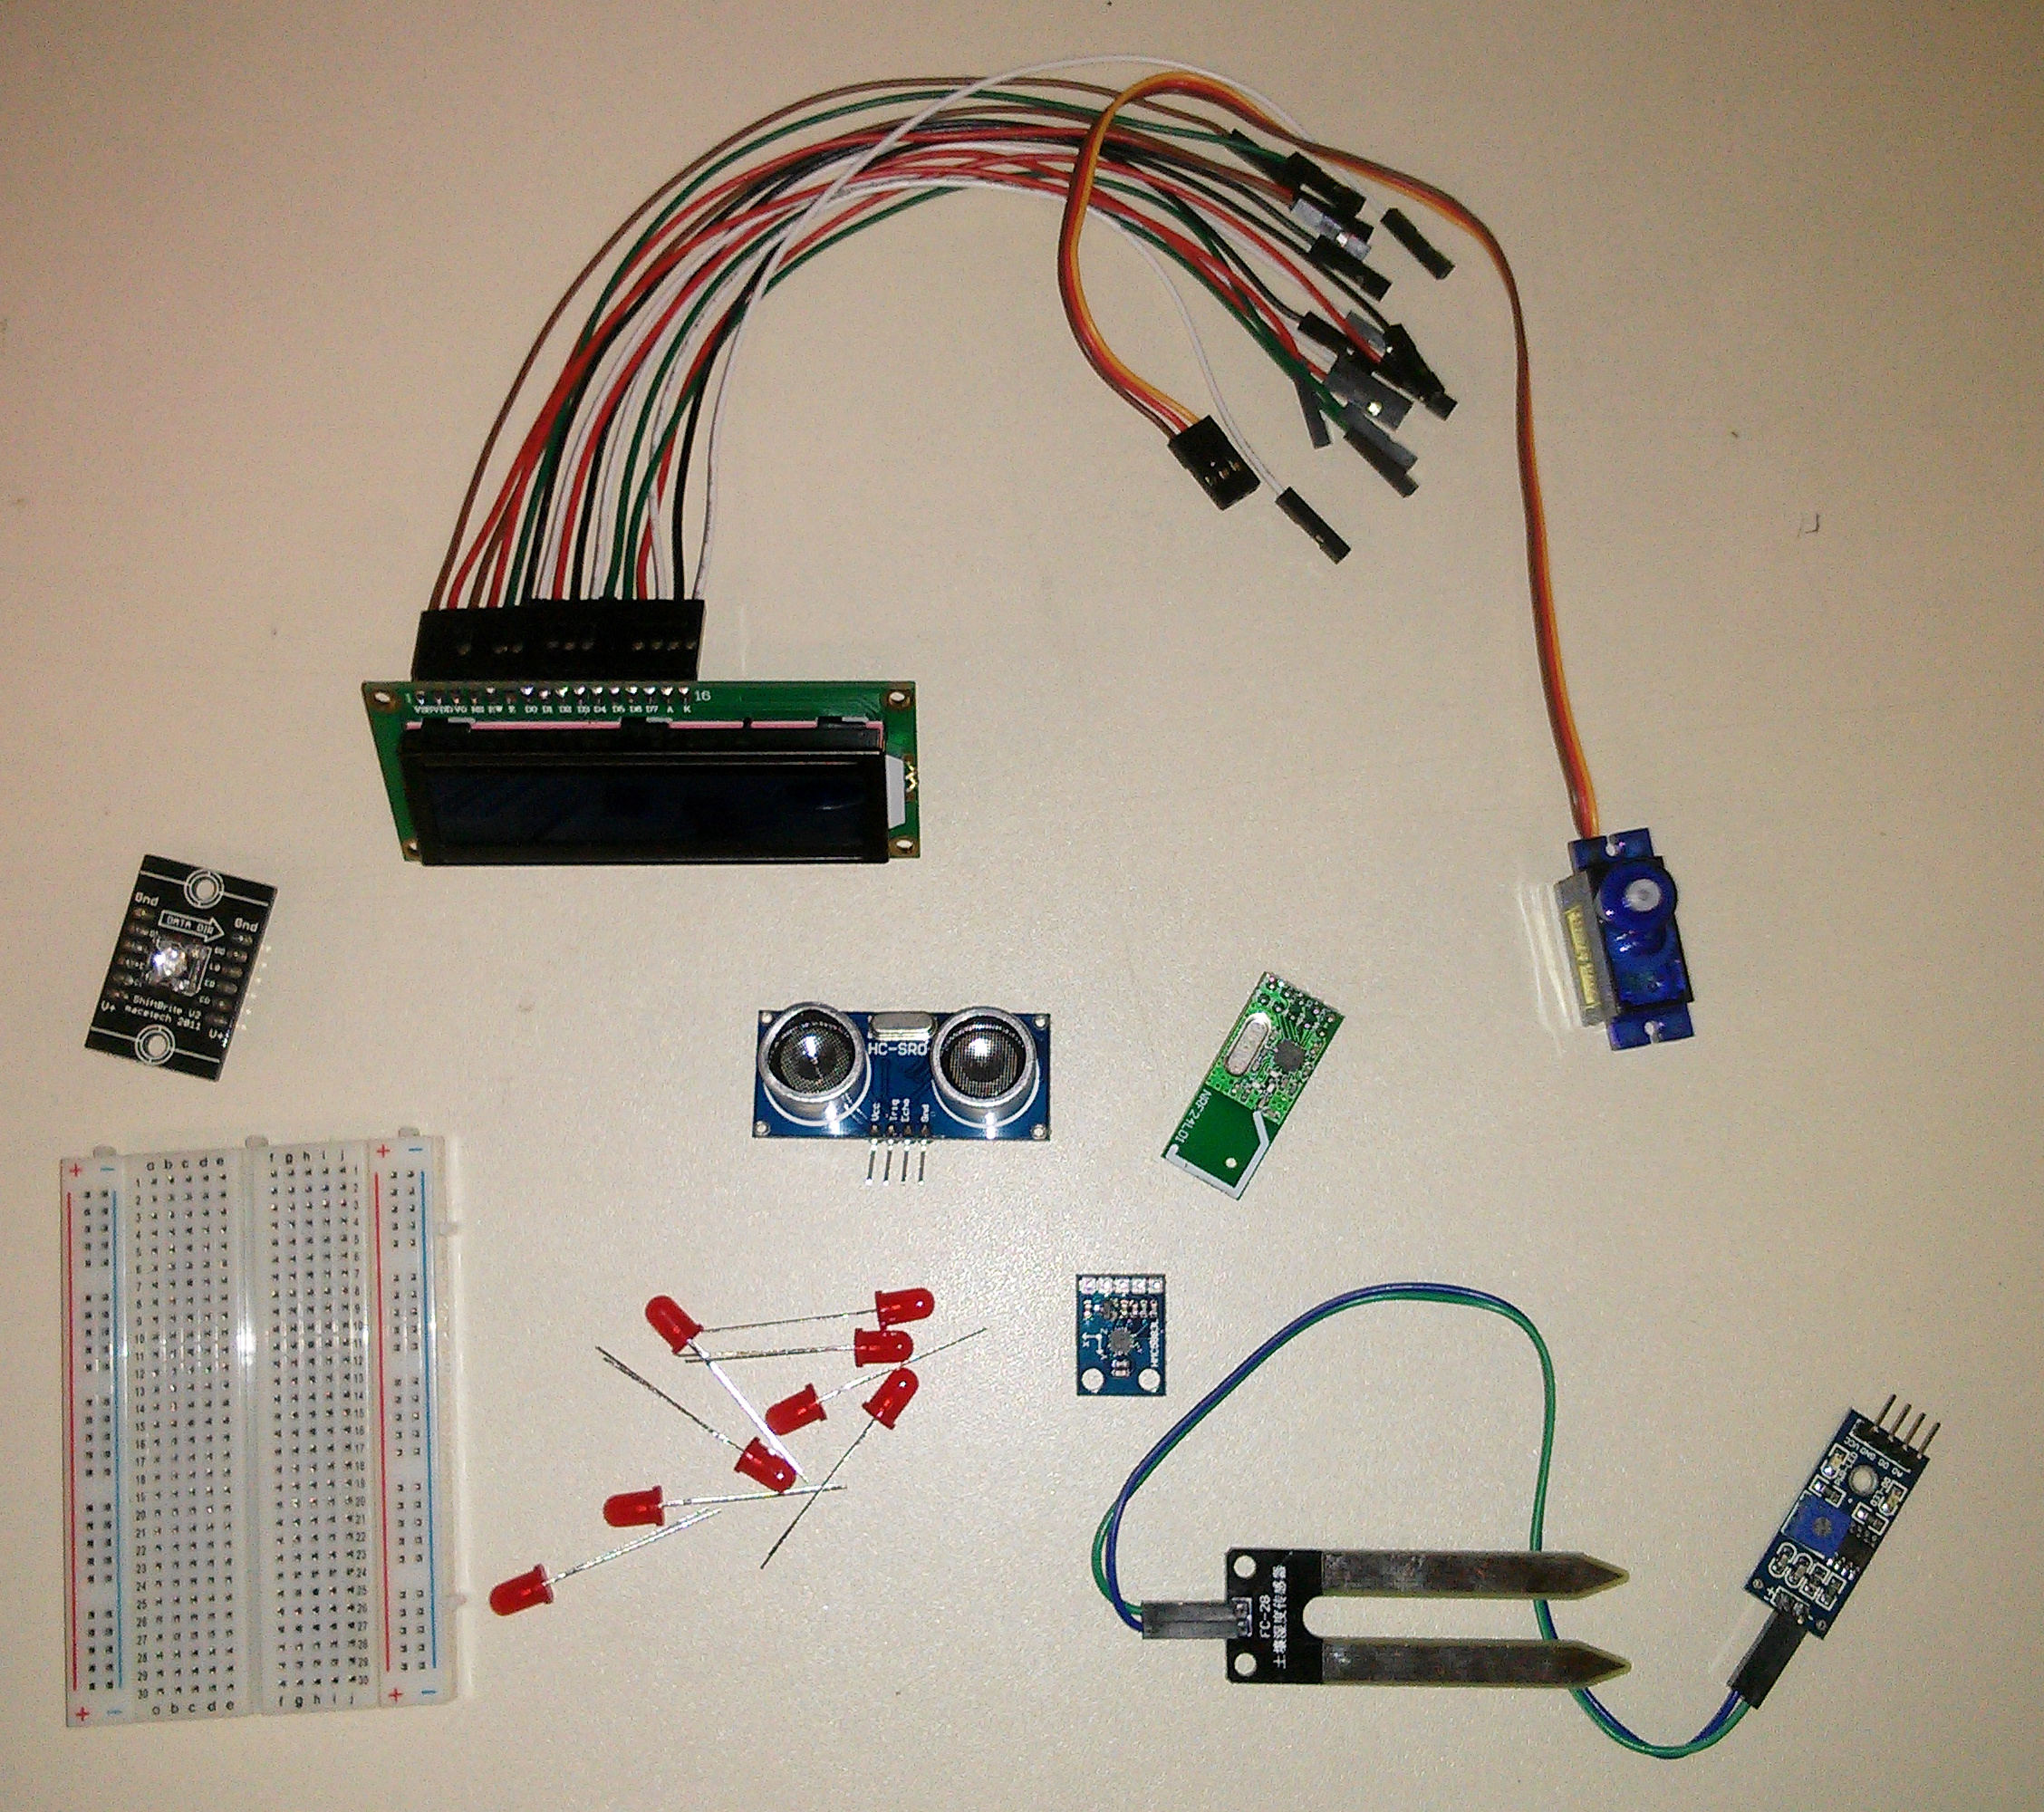
\includegraphics[width=0.6\textwidth]{bauteile.jpg}
	\end{figure}
\end{frame}

\begin{frame}{Resultat}
	\begin{itemize}
		\item Projekte aus 5 kleinen Gruppen
		\item verschieden fertig
	\end{itemize}
	\begin{center}
		\visible<2>{\Huge \alert{STOP:} Demo time}
	\end{center}
\end{frame}

\begin{frame}{Danke}
	\begin{center}
		\visible{\Huge Danke}
	\end{center}
	\begin{itemize}
		\item TobiX
		\item ike
		\item gordin
		\item zakx
	\end{itemize}
\end{frame}

\end{document}
